\documentclass[tikz,convert={outfile=\jobname.svg}]{standalone}
\usepackage{pgf} 
\usepackage{amsmath}
\usepackage{ifthen}
\usetikzlibrary{positioning}
\usetikzlibrary{fit}
\usetikzlibrary{calc}

\begin{document}
\newcommand{\drawRCC}{
  
\begin{tikzpicture}
    \fill[black] (0,0) rectangle (3, 4);
    \clip (0,0) rectangle (3, 4); 
    \fill[gray] (0, 0.2) arc[start angle=-90, end angle=90, radius=1.8] -- cycle;
    \draw[white, ultra thick] (0, 0.2) arc[start angle=-90, end angle=90, radius=1.8];
    \node[white, anchor=north east, inner sep=2, outer sep=2] at (current bounding box.north east) {RCC};
    \draw[white, ultra thick] (0,0) rectangle (3, 4);
  \end{tikzpicture}
}

\newcommand{\drawMaskedRCC}[4]{
  \pgfmathsetseed{#1}
  \begin{tikzpicture}
    \fill[black] (0,0) rectangle (3, 4);
    \clip (0,0) rectangle (3, 4); 
    \fill[gray] (0, 0.2) arc[start angle=-90, end angle=90, radius=1.8] -- cycle;
    \draw[white, ultra thick] (0, 0.2) arc[start angle=-90, end angle=90, radius=1.8];
    \node[white, anchor=north east] at (3, 4) {RCC};
    \draw[white, ultra thick] (0,0) rectangle (3, 4);
    \foreach \x in {0, 1, 2} {
      \foreach \y in {0, 1, 2, 3} {
        \draw[white, very thin] (\x, \y) rectangle (\x+1, \y+1);
        \pgfmathsetmacro{\rand}{random}
        \ifdim \rand pt < \dimexpr#2 pt\relax
          \fill[#3, opacity=#4] (\x, \y) rectangle (\x+1, \y+1);
        \else
          \fill[black] (\x, \y) rectangle (\x+1, \y+1);
        \fi
      }
    }
  \end{tikzpicture}
}

\newcommand{\drawMLP}{
  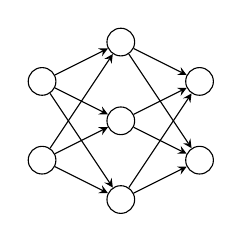
\begin{tikzpicture}
    % Input layer
    \foreach \i in {1, 2} {
      \node[circle, draw=black, fill=white, minimum size=10pt, inner sep=0pt] (input\i) at (0, -\i-0.5) {};
    }

    % Hidden layer
    \foreach \i in {1, 2, 3} {
      \node[circle, draw=black, fill=white, minimum size=10pt, inner sep=0pt] (hidden\i) at (1, -\i) {};
    }

    % Output layer
    \foreach \i in {1, 2} {
      \node[circle, draw=black, fill=white, minimum size=10pt, inner sep=0pt] (output\i) at (2, -\i-0.5) {};
    }

    % Connections from input to hidden layer
    \foreach \i in {1, 2} {
      \foreach \j in {1, 2, 3} {
        \draw[->, black, >=stealth] (input\i) -- (hidden\j);
      }
    }

    % Connections from hidden to output layer
    \foreach \i in {1, 2, 3} {
      \foreach \j in {1, 2} {
        \draw[->, black, >=stealth] (hidden\i) -- (output\j);
      }
    }
  \end{tikzpicture}
}

\newcommand{\drawFeatures}[3]{
  \begin{tikzpicture}
  \pgfmathsetseed{#1}
  \foreach \i in {0, ..., #2} {
    \node at (\i*0.8, 0) {
      $\color{#3}\scriptsize\begin{bmatrix}
        \pgfmathsetmacro{\rand}{rnd*9.9}
        \pgfmathprintnumber[fixed, precision=1]{\rand} \\
        \pgfmathsetmacro{\rand}{rnd*9.9}
        \pgfmathprintnumber[fixed, precision=1]{\rand} \\
        \vdots \\
        \pgfmathsetmacro{\rand}{rnd*9.9}
        \pgfmathprintnumber[fixed, precision=1]{\rand} \\
        \pgfmathsetmacro{\rand}{rnd*9.9}
        \pgfmathprintnumber[fixed, precision=1]{\rand}
      \end{bmatrix}$
    };
  }
  \end{tikzpicture}
}


\newcommand{\drawPosEnc}{
  \begin{tikzpicture}
  \node[circle, draw=black, minimum size=6cm] (circle) at (0, 0) {};
  \draw[black] (-3, 0) sin (-1.5, -1) cos (0, 0) sin (1.5, 1) cos (3, 0);
  \end{tikzpicture}
}
\tikzset{every picture/.style={/utils/exec={\sffamily}}}

\begin{tikzpicture}
    % Input image
    \node[name=rcc] at (0, 0){\drawRCC};
    \node[below=0.5cm of rcc.south, anchor=center] {Input Image};

    % Patch embedding
    \node[name=patch_embedding] at (4, 0){\drawMLP};
    \node[below=0.5cm of patch_embedding.south, anchor=center] {Patch Embedding};
    \draw[->, thick, black, >=stealth, line width=1.5pt] (rcc) -- (patch_embedding);

    % Dynamic features
    \node[name=dynamic] at (8, 0){\drawMaskedRCC{3}{1.0}{red}{0.2}{4}{6}};
    \draw[->, thick, black, >=stealth, line width=1.5pt] (patch_embedding) -- (dynamic);
    \node[above=0.5cm of dynamic.north, anchor=center] {Embeddings};

    % Fixed features
    \node[name=fixed] at (8, -8){\drawMaskedRCC{3}{1.0}{green}{0.2}{3}{4}};
    \node[below=0.5cm of fixed.south, anchor=center] {Fixed Embeddings};
    \draw[->, thick, black, >=stealth, line width=1.5pt] (dynamic) -- (fixed) 
        node[name=midpool, midway, anchor=center, right] {\rotatebox{-90}{Adaptive Pooling}};

    % Position encoding
    \node[name=position_encoding, right=1.5cm of midpool.east, anchor=center, scale=0.1, outer sep=1cm] {\drawPosEnc};

    % Fixed Block
    \node[name=block2, right=1cm of fixed.east, anchor=west] {\drawDetailedDecoderBlock{t}};
    \node[below=0.5cm of block2.south, anchor=center] {Transformer Decoder};
    \draw[->, thick, black, >=stealth, line width=1.5pt] (fixed) -- (block2);
    \node[below=0.5cm of block2.south east, anchor=east] {Repeat Nx};

    % Dynamic Block
    \node[name=block1, right=1cm of dynamic.east, anchor=west] {\drawDetailedDecoderBlock{f}};
    \node[above=0.5cm of block1.north, anchor=center] {Transformer Decoder};
    \draw[->, thick, black, >=stealth, line width=1.5pt] (dynamic) -- (block1);
    \node[above=0.5cm of block1.north east, anchor=east] {Repeat Nx};

    \draw[->, thick, black, >=stealth, line width=1.5pt] 
        (position_encoding) 
        to[out=90, in=180]
        (block1);
    \draw[->, thick, black, >=stealth, line width=1.5pt] 
        (position_encoding) 
        to[out=270, in=180]
        (block2);

    % Output scale
    \node[name=output_scale, right=1cm of block1.east, anchor=west] {\drawLayerBlock{Layer Scale}{gray!20}};
    \draw[->, thick, black, >=stealth, line width=1.5pt] (block1) -- (output_scale);

    % Output
    \node[name=output, right=4cm of output_scale.east, anchor=west] {\drawMaskedRCC{3}{1.0}{blue}{0.2}{4}{6}};
    \draw[->, thick, black, >=stealth, line width=1.5pt] (output_scale) -- (output);
    \node[above=0.5cm of output.north, anchor=center] {Output Features};

    % Resize and add
    \draw[->, thick, black, >=stealth, line width=1.5pt] 
        (block2) 
        to[out=0, in=270]
        node[near end, left] {Resize and Add}
        (output);

    % Cross attention connections
    \draw[->, thick, red, >=stealth, line width=1.5pt] 
        ($(block1.south west)+(3.25cm,0)$) 
        -- ($(block2.north west)+(3.25cm,0)$);
    \draw[->, thick, red, >=stealth, line width=1.5pt] 
        ($(block2.north west)+(8.9cm,0)$)
        -- ($(block1.south west)+(8.9cm,0)$);


  

\end{tikzpicture}
\end{document}